\documentclass[conference]{IEEEtran}
\IEEEoverridecommandlockouts
\usepackage{amsmath}
\usepackage[T1]{fontenc}
\usepackage{newtxtext,newtxmath}
\usepackage{graphicx}
\usepackage{booktabs}
\usepackage{array}
\usepackage{tikz}
\usetikzlibrary{arrows.meta,positioning,calc,fit}
\usepackage[hidelinks]{hyperref}
\hypersetup{
  pdftitle={Design and Verification of a Parameterized Systolic Array Accelerator for Matrix Multiplication},
  pdfauthor={Gargi, Agrima, Bhawana, Deepak, Dev (Group Kamlesh)},
  pdfsubject={Systolic Array Matrix Multiplication Accelerator},
  pdfkeywords={systolic array, matrix multiplication, hardware accelerator, Verilog, processing element},
  pdfcreator={Group Kamlesh},
  pdfproducer={Group Kamlesh}
}

\begin{document}

\title{Design and Verification of a Parameterized Systolic Array Accelerator for Matrix Multiplication}

\author{\IEEEauthorblockN{Gargi, Agrima, Bhawana, Deepak, Dev}
\IEEEauthorblockA{Group Kamlesh}}

\maketitle

\begin{abstract}
Matrix multiplication dominates the computational cost of modern machine-learning
workloads, which has made systolic arrays a standard building block of deep-learning
accelerators. This paper presents the design and verification of a parameterized
output-stationary systolic array accelerator for signed integer matrix multiplication,
implemented in Verilog. The accelerator is composed of five modules: a multiply--accumulate
(MAC) unit, a processing element (PE) with registered operand forwarding, an
$N\times N$ systolic array generated from the PE, an input buffer with a skewed
matrix-streaming interface, and a finite-state-machine (FSM) controller that sequences
initialization, operand feeding, pipeline flushing and completion. Each module was verified
independently, and the complete system was verified for $2\times2$, $3\times3$ and $4\times4$
matrices, with every output matching a reference product. A multiplication of two
$N\times N$ matrices completes in $3N-1$ compute cycles, so the $4\times4$ configuration
performs 64 MAC operations in 11 cycles, an average of 5.82 MAC operations per cycle and a
$5.8\times$ cycle-count reduction relative to a single-MAC sequential implementation. All 16
testbenches pass in Icarus Verilog simulation.
\end{abstract}

\begin{IEEEkeywords}
systolic array, matrix multiplication, hardware accelerator, multiply--accumulate, Verilog, output-stationary dataflow
\end{IEEEkeywords}

\section{Introduction}
Dense matrix multiplication is the central operation in neural-network inference and
training: fully connected layers are matrix products, and convolutions are routinely lowered
to matrix products. General-purpose processors perform this computation largely
sequentially, and their performance is often limited by memory bandwidth rather than by
arithmetic. A systolic array addresses both problems. It arranges many simple processing
elements in a regular grid in which data flows rhythmically from neighbour to neighbour, so
that every operand fetched from memory is reused by many PEs and all PEs compute in parallel
using only local connections.

This project designs, implements and verifies a complete systolic array accelerator in
Verilog. The contributions are:
\begin{itemize}
\item a parameterized MAC unit and PE with configurable operand and accumulator widths;
\item an $N\times N$ output-stationary systolic array built with generate loops, so the
same RTL instantiates any array size;
\item an input buffer and matrix interface that store both operand matrices and stream them
into the array with the diagonal skew required for correct timing;
\item an FSM controller that coordinates the buffer, the interface and the array; and
\item a layered verification flow, from unit tests to full-system tests at three array
sizes, together with a cycle-level performance analysis.
\end{itemize}

\section{Literature Review}
\subsection{Origins of Systolic Arrays}
Systolic arrays were introduced by Kung and Leiserson~\cite{kung1979} as a way to map
regular algorithms such as matrix multiplication and LU decomposition onto VLSI. Kung later
summarized the motivation~\cite{kung1982}: by passing data through a chain of PEs instead of
returning to memory after every operation, a systolic design performs many operations per
memory access and balances computation against I/O bandwidth, while the modular, locally
connected structure suits VLSI layout.

\subsection{Systolic Arrays in Deep-Learning Accelerators}
The approach regained prominence with deep learning. Google's first Tensor Processing Unit
(TPU)~\cite{jouppi2017} is built around a $256\times256$ systolic matrix-multiply unit of 65,536
8-bit MACs with a peak throughput of 92 TOPS. It uses a weight-stationary dataflow in which
weights are preloaded into the PEs while activations stream through the array. Eyeriss~\cite{chen2016,chen2017}
uses a 168-PE spatial array with a row-stationary dataflow that maximizes local data reuse to
reduce energy, showing that data movement rather than arithmetic dominates accelerator
energy.

\subsection{Dataflow Taxonomy}
Sze \emph{et al.}~\cite{sze2017} classify accelerator dataflows by which operand stays fixed
in each PE: weight-stationary, output-stationary, input-stationary and row-stationary.
In an output-stationary array each PE owns one output element and accumulates its partial
sum locally, while both input matrices stream past it. This removes the need to move partial
sums between PEs and gives a simple, regular design. SCALE-Sim~\cite{samajdar2018} provides
a cycle-accurate model of systolic arrays and compares these dataflows, showing how array
shape and dataflow affect utilization and runtime. The Gemmini generator~\cite{genc2021}
produces systolic accelerators that support both weight-stationary and output-stationary
dataflows, demonstrating that both are practical in silicon.

\subsection{Position of This Work}
This project adopts the output-stationary dataflow for its simplicity: partial sums never
leave the PE, and the array produces a complete result matrix in place. The design focuses on
an RTL implementation that is parameterized in array size and data width, with each block
verified independently and in integration. It is written in IEEE~1364-2005
Verilog~\cite{ieee1364} and simulated with Icarus Verilog~\cite{icarus}.

\section{Proposed Solution}
\subsection{System Architecture}
Fig.~\ref{fig:system} shows the complete accelerator. Operand pairs are loaded sequentially
into the input buffer. When the buffer reports \texttt{buffer\_ready} and \texttt{start} is
asserted, the controller resets the array, enables the matrix interface to stream skewed
operands for $2N-1$ cycles, holds the array enabled for $N$ further flush cycles, and asserts
\texttt{done}. The result matrix is then available on \texttt{acc\_out}.

\begin{figure}[t]
\centering
\resizebox{\columnwidth}{!}{%
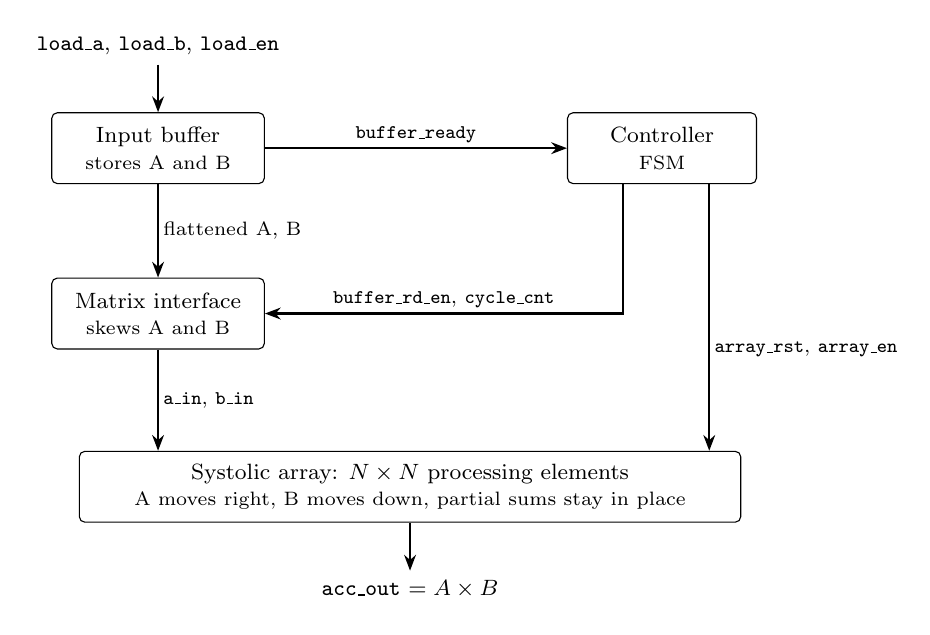
\begin{tikzpicture}[
  blk/.style={draw, rounded corners=2pt, align=center, font=\footnotesize, minimum height=9mm, inner sep=3pt},
  arr/.style={-{Stealth[length=2mm]}, thick},
  lbl/.style={font=\scriptsize, inner sep=1.5pt}]
\node[blk, minimum width=27mm] (buf) at (0,0) {Input buffer\\\scriptsize stores A and B};
\node[blk, minimum width=24mm] (ctl) at (6.4,0) {Controller\\\scriptsize FSM};
\node[blk, minimum width=27mm] (mif) at (0,-2.1) {Matrix interface\\\scriptsize skews A and B};
\node[blk, minimum width=84mm] (arr) at (3.2,-4.3) {Systolic array: $N\times N$ processing elements\\\scriptsize A moves right, B moves down, partial sums stay in place};
\node[font=\footnotesize] (in) at (0,1.3) {\texttt{load\_a}, \texttt{load\_b}, \texttt{load\_en}};
\node[font=\footnotesize] (out) at (3.2,-5.6) {\texttt{acc\_out} $= A\times B$};
\draw[arr] (in) -- (buf);
\draw[arr] (buf) -- node[lbl, above]{\texttt{buffer\_ready}} (ctl);
\draw[arr] (buf) -- node[lbl, right]{flattened A, B} (mif);
\draw[arr] (ctl.south) ++(-0.5,0) coordinate (c1) -- (c1 |- mif.east) -- node[lbl, above, pos=0.5]{\texttt{buffer\_rd\_en}, \texttt{cycle\_cnt}} (mif.east);
\draw[arr] (mif.south) -- node[lbl, right]{\texttt{a\_in}, \texttt{b\_in}} (mif.south |- arr.north);
\draw[arr] (ctl.south) ++(0.6,0) coordinate (c2) -- node[lbl, right, pos=0.62]{\texttt{array\_rst}, \texttt{array\_en}} (c2 |- arr.north);
\draw[arr] (arr) -- (out);
\end{tikzpicture}}
\caption{Top-level architecture of the accelerator.}
\label{fig:system}
\end{figure}

\subsection{MAC Unit and Processing Element}
The MAC unit multiplies two signed \texttt{DATA\_WIDTH}-bit operands and adds the
$2\cdot$\texttt{DATA\_WIDTH}-bit product to a signed \texttt{ACC\_WIDTH}-bit accumulator on each
rising clock edge while \texttt{en} is high: $\mathit{acc} \leftarrow \mathit{acc} + a\cdot b$.
A synchronous active-high reset clears the accumulator, and the accumulator holds its value
when \texttt{en} is low. The default widths are 8-bit operands and a 32-bit accumulator.
Overflow wraps around in two's complement; no saturation logic is used.

The PE wraps the MAC unit and adds two registers that forward its inputs to its neighbours:
\texttt{a\_out} $\leftarrow$ \texttt{a\_in} to the PE on the right and \texttt{b\_out}
$\leftarrow$ \texttt{b\_in} to the PE below. The MAC consumes \texttt{a\_in} and \texttt{b\_in}
directly, so each operand is used in the cycle it arrives and passed on one cycle later.

\subsection{Parameterized Systolic Array}
The array instantiates $N^2$ PEs with nested Verilog \texttt{generate} loops, so
\texttt{N}, \texttt{DATA\_WIDTH} and \texttt{ACC\_WIDTH} are module parameters and no wiring
is written by hand. Internal unpacked wire arrays form the forwarding mesh: the A operand for
row $i$ enters PE$[i][0]$ and moves right, and the B operand for column $j$ enters PE$[0][j]$
and moves down (Fig.~\ref{fig:array}). The ports are flattened vectors so the module remains
compatible with Verilog-2001 and Verilog-2005: \texttt{a\_in} and \texttt{b\_in} are
$N\cdot$\texttt{DATA\_WIDTH} bits wide, and \texttt{acc\_out} is
$N^2\cdot$\texttt{ACC\_WIDTH} bits wide, with PE$[i][j]$ at word index $iN+j$.

\begin{figure}[t]
\centering
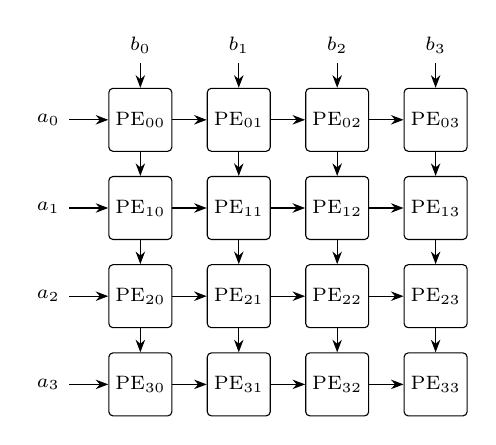
\begin{tikzpicture}[
  pe/.style={draw, rounded corners=1.5pt, minimum size=8mm, font=\scriptsize, inner sep=0pt},
  ar/.style={-{Stealth[length=1.6mm]}}]
\foreach \i in {0,1,2,3} {
  \foreach \j in {0,1,2,3} {
    \node[pe] (p\i\j) at (\j*1.25, -\i*1.12) {PE$_{\i\j}$};
  }
  \node[font=\scriptsize, anchor=east] (a\i) at (-0.9, -\i*1.12) {$a_{\i}$};
  \draw[ar] (a\i) -- (p\i0);
}
\foreach \j in {0,1,2,3} {
  \node[font=\scriptsize] (b\j) at (\j*1.25, 0.95) {$b_{\j}$};
  \draw[ar] (b\j) -- (p0\j);
}
\foreach \i in {0,1,2,3} {
  \foreach \j/\k in {0/1,1/2,2/3} { \draw[ar] (p\i\j) -- (p\i\k); }
}
\foreach \j in {0,1,2,3} {
  \foreach \i/\k in {0/1,1/2,2/3} { \draw[ar] (p\i\j) -- (p\k\j); }
}
\end{tikzpicture}
\caption{$4\times4$ output-stationary array. A operands move right and B operands move down
through registered links. PE$_{ij}$ accumulates $C[i][j]$ in place.}
\label{fig:array}
\end{figure}

\subsection{Input Buffer and Skewed Matrix Interface}
The input buffer stores one A element and one B element per clock while \texttt{load\_en} is
high. After all $N^2$ pairs are stored it asserts \texttt{buffer\_ready}, and it presents
both matrices as flattened vectors. The matrix interface is combinational. Using the
controller's \texttt{cycle\_cnt}, it drives row $i$ of the array with $A[i][t-i]$ and column $j$
with $B[t-j][j]$ in feed cycle $t$, and drives zero when the index is out of range or when
\texttt{buffer\_rd\_en} is low.

This skew is what makes the array compute the correct product. Element $A[i][k]$ enters row $i$
in cycle $k+i$ and needs $j$ register hops to reach PE$[i][j]$, arriving in cycle $i+j+k$.
Element $B[k][j]$ enters column $j$ in cycle $k+j$ and needs $i$ hops, so it also arrives in
cycle $i+j+k$. Every pair needed for
\begin{equation}
C[i][j] = \sum_{k=0}^{N-1} A[i][k]\,B[k][j]
\end{equation}
therefore meets at PE$[i][j]$ in the same cycle. The last product, with $i=j=k=N-1$, arrives in
cycle $3N-3$.

\subsection{Controller}
The controller is a four-state FSM (Fig.~\ref{fig:fsm}) with an active-low reset. In
\textsc{Idle} it waits for both \texttt{start} and \texttt{buffer\_ready}. \textsc{Init}
asserts \texttt{array\_rst} for one cycle to clear every accumulator and forwarding register.
\textsc{Compute} asserts \texttt{array\_en} and increments \texttt{cycle\_cnt}. It asserts
\texttt{buffer\_rd\_en} during the $2N-1$ feed cycles and deasserts it during the $N$ flush
cycles, in which zeros enter the array while the remaining products propagate. After $3N-1$
compute cycles the FSM enters \textsc{Done}, asserts \texttt{done} for one cycle, and returns
to \textsc{Idle}. The $3N-1$-cycle window fully covers the final product, which arrives in cycle
$3N-3$.

\begin{figure}[t]
\centering
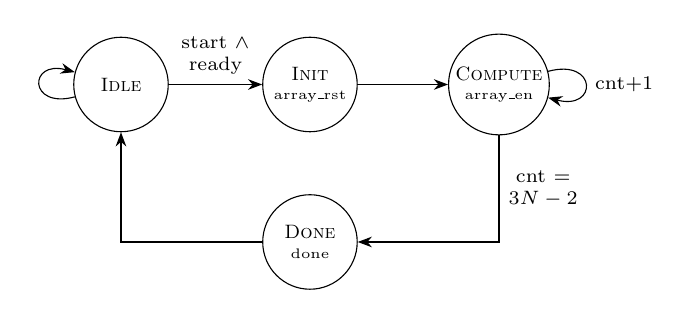
\begin{tikzpicture}[
  st/.style={draw, circle, minimum size=12mm, font=\scriptsize, align=center, inner sep=1pt},
  ar/.style={-{Stealth[length=1.8mm]}},
  lbl/.style={font=\scriptsize, align=center}]
\node[st] (idle) at (0,0) {\textsc{Idle}};
\node[st] (init) at (2.4,0) {\textsc{Init}\\[-1pt]\tiny array\_rst};
\node[st] (comp) at (4.8,0) {\textsc{Compute}\\[-1pt]\tiny array\_en};
\node[st] (done) at (2.4,-2.0) {\textsc{Done}\\[-1pt]\tiny done};
\draw[ar] (idle) -- node[lbl, above]{start $\wedge$\\ready} (init);
\draw[ar] (init) -- (comp);
\draw[ar] (comp) |- node[lbl, pos=0.25, right]{cnt $=$\\$3N-2$} (done);
\draw[ar] (done) -| (idle);
\draw[ar] (idle) edge[loop left, looseness=5] (idle);
\draw[ar] (comp) edge[loop right, looseness=5] node[lbl, right]{cnt$+1$} (comp);
\end{tikzpicture}
\caption{Controller FSM. \texttt{buffer\_rd\_en} is high in the first $2N-1$ compute cycles.}
\label{fig:fsm}
\end{figure}

\subsection{Verification Methodology}
Verification was layered so that faults could be isolated to a single block. Unit testbenches
check the MAC unit (accumulation, hold, reset, parameterized widths and two's-complement
overflow) and the PE (signed arithmetic, forwarding, back-to-back operations and stress
sequences). Integration testbenches check a hand-wired $2\times2$ array, the parameterized
$4\times4$ array driven with skewed inputs, the input buffer, the matrix interface, the
controller, and the controller combined with the array. A full-system testbench connects all
modules, loads deterministic signed matrices, compares every accumulator with a reference
product computed in the testbench, and checks the controller at every cycle: \texttt{cycle\_cnt}
must match the expected count and \texttt{buffer\_rd\_en} must be high exactly during the feed
window. The full-system test was run for $N=2$, $3$ and $4$.

\section{Results}
\subsection{Functional Verification}
All 16 testbenches pass. In the full-system test every output matched the reference product
for all three array sizes (Table~\ref{tab:perf}). For $N=4$ the operands are
\[
A=\begin{bmatrix}-6&-1&4&-4\\1&6&-2&3\\-5&0&5&-3\\2&-6&-1&4\end{bmatrix},\;
B=\begin{bmatrix}-5&-2&1&4\\-1&2&5&-3\\3&-5&-2&1\\-4&-1&2&5\end{bmatrix},
\]
and the accelerator produced
\[
C=\begin{bmatrix}59&-6&-27&-37\\-29&17&41&-1\\52&-12&-21&-30\\-23&-15&-18&45\end{bmatrix},
\]
which is exactly $A\times B$. These operands mix positive and negative values, so they also
exercise signed multiplication and accumulation.

Fig.~\ref{fig:wave} shows the $4\times4$ simulation waveform. After \texttt{start}, the
controller pulses \texttt{array\_rst} for one cycle and raises \texttt{array\_en}.
\texttt{buffer\_rd\_en} stays high for the 7 feed cycles and low for the 4 flush cycles, and
\texttt{done} rises after 11 compute cycles. $C[0][0]$, computed by the top-left PE, settles
first, at 59. $C[3][3]$, computed by the bottom-right PE, receives its last product in compute
cycle 9 ($3N-3$) and settles at 45.

\begin{figure*}[t]
\centering
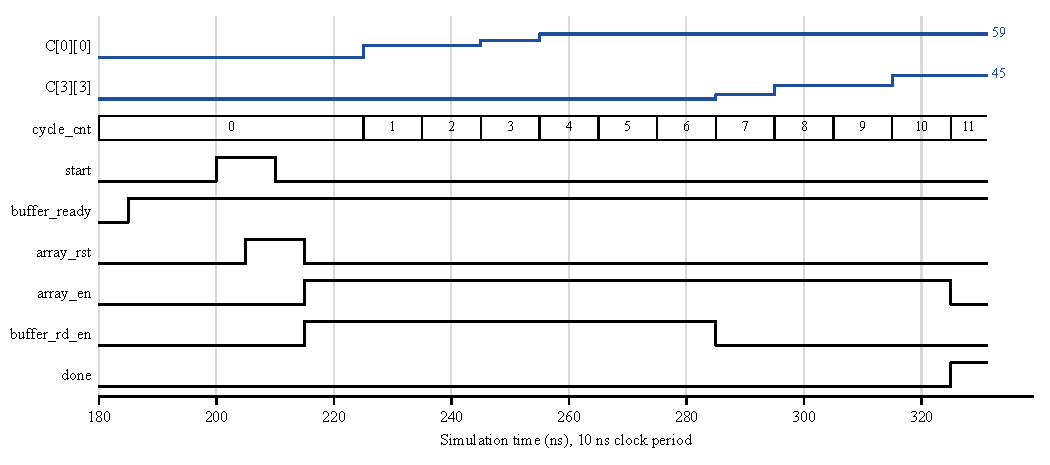
\includegraphics[width=\textwidth]{fig_waveform.pdf}
\caption{Full-system simulation waveform for $N=4$. The controller steps through 7 feed cycles
(\texttt{buffer\_rd\_en} high) and 4 flush cycles before asserting \texttt{done}. The traces at
the top show the accumulators of the first and last PEs reaching their final values, 59 and 45.}
\label{fig:wave}
\end{figure*}

\subsection{Performance Analysis}
Table~\ref{tab:perf} lists the cycle counts measured in simulation. A product of two
$N\times N$ matrices needs $N^3$ scalar MAC operations. A sequential datapath with one MAC
unit needs at least $N^3$ cycles, while the systolic array needs $3N-1$ compute cycles, or
$3N$ including the initialization cycle. The average throughput is therefore
\begin{equation}
\text{MAC/cycle} = \frac{N^3}{3N-1},
\end{equation}
which grows roughly as $N^2/3$. For $N=4$, the cycle count falls from 64 to 11, a $5.8\times$
reduction, using 16 PEs with a peak capacity of $N^2=16$ MACs per cycle. The gap between
average and peak throughput comes from the fill and drain phases of the skewed schedule. It
shrinks relative to total work when larger matrices are tiled over the array or when
consecutive multiplications are overlapped.

\begin{table}[t]
\centering
\caption{Full-System Simulation Results}
\label{tab:perf}
\setlength{\tabcolsep}{4.5pt}
\begin{tabular}{@{}cccccc@{}}
\toprule
Array & Outputs & Compute & MAC ops & Avg. & Sequential\\
size & checked & cycles & ($N^3$) & MAC/cycle & speed-up\\
\midrule
$2\times2$ & 4 & 5 & 8 & 1.600 & $1.6\times$\\
$3\times3$ & 9 & 8 & 27 & 3.375 & $3.4\times$\\
$4\times4$ & 16 & 11 & 64 & 5.818 & $5.8\times$\\
\bottomrule
\end{tabular}
\end{table}

\subsection{Limitations}
The results are cycle counts from RTL simulation. The design has not been synthesized, so
area, maximum clock frequency and power have not been measured. Accumulator overflow wraps
around rather than saturating, and the array processes one $N\times N$ product at a time
without tiling for larger matrices.

\section{Individual Contributions}
The accelerator was partitioned into five blocks with defined interfaces so that members could
work in parallel and integrate through version control. Contributions are listed in
Table~\ref{tab:contrib} and are reflected in the commit history of the project repository.

\begin{table}[t]
\centering
\caption{Individual Contributions}
\label{tab:contrib}
\renewcommand{\arraystretch}{1.15}
\begin{tabular}{@{}>{\raggedright\arraybackslash}p{0.6in}>{\raggedright\arraybackslash}p{2.6in}@{}}
\toprule
Member & Contribution\\
\midrule
Gargi & MAC unit and processing element (\texttt{mac\_unit.v}, \texttt{processing\_element.v}); width parameterization; MAC, PE, stress, overflow, back-to-back and $2\times2$ integration testbenches; PE interface specification.\\
Agrima & Parameterized $N\times N$ systolic array (\texttt{systolic\_array.v}) with generate-based PE mesh and flattened ports; $4\times4$ array integration testbench; array architecture documentation and verification report.\\
Bhawana & Input buffer and skewed matrix interface (\texttt{input\_buffer.v}, \texttt{matrix\_interface.v}); buffer, interface and integration testbenches; design report and waveforms.\\
Deepak & FSM controller (\texttt{systolic\_controller.v}); controller unit testbench and controller--array integration testbench; controller architecture and interface specification.\\
Dev & Full-system verification testbench for $N=2$, $3$, $4$ with per-cycle control checks; performance analysis of latency and throughput; verification and performance report.\\
\bottomrule
\end{tabular}
\end{table}

\section{Conclusion and Future Work}
This project implemented and verified a parameterized output-stationary systolic array
accelerator for signed matrix multiplication in Verilog. The modular design (MAC unit, PE,
array, buffered skewed interface and FSM controller) computes an $N\times N$ product in
$3N-1$ compute cycles and passed all unit, integration and full-system tests for $N$ up to 4.
Planned extensions are FPGA synthesis to obtain area, frequency and power figures, tiling to
multiply matrices larger than the array, overlapping consecutive multiplications to hide fill
and drain latency, saturating arithmetic, and a comparison with a weight-stationary variant.

\begin{thebibliography}{10}
\bibitem{kung1979}
H.~T. Kung and C.~E. Leiserson, ``Systolic arrays (for VLSI),'' in \emph{Sparse Matrix
Proceedings 1978}, I.~S. Duff and G.~W. Stewart, Eds. Philadelphia, PA, USA: SIAM, 1979,
pp. 256--282.

\bibitem{kung1982}
H.~T. Kung, ``Why systolic architectures?'' \emph{Computer}, vol.~15, no.~1, pp. 37--46,
Jan. 1982.

\bibitem{jouppi2017}
N.~P. Jouppi \emph{et al.}, ``In-datacenter performance analysis of a tensor processing
unit,'' in \emph{Proc. 44th Annu. Int. Symp. Comput. Archit. (ISCA)}, 2017, pp. 1--12.

\bibitem{chen2016}
Y.-H. Chen, J. Emer, and V. Sze, ``Eyeriss: A spatial architecture for energy-efficient
dataflow for convolutional neural networks,'' in \emph{Proc. 43rd Annu. Int. Symp. Comput.
Archit. (ISCA)}, 2016, pp. 367--379.

\bibitem{chen2017}
Y.-H. Chen, T. Krishna, J.~S. Emer, and V. Sze, ``Eyeriss: An energy-efficient
reconfigurable accelerator for deep convolutional neural networks,'' \emph{IEEE J.
Solid-State Circuits}, vol.~52, no.~1, pp. 127--138, Jan. 2017.

\bibitem{sze2017}
V. Sze, Y.-H. Chen, T.-J. Yang, and J.~S. Emer, ``Efficient processing of deep neural
networks: A tutorial and survey,'' \emph{Proc. IEEE}, vol.~105, no.~12, pp. 2295--2329,
Dec. 2017.

\bibitem{samajdar2018}
A. Samajdar, Y. Zhu, P. Whatmough, M. Mattina, and T. Krishna, ``SCALE-Sim: Systolic CNN
accelerator simulator,'' arXiv:1811.02883, 2018.

\bibitem{genc2021}
H. Genc \emph{et al.}, ``Gemmini: Enabling systematic deep-learning architecture evaluation
via full-stack integration,'' in \emph{Proc. 58th ACM/IEEE Design Autom. Conf. (DAC)}, 2021,
pp. 769--774.

\bibitem{ieee1364}
\emph{IEEE Standard for Verilog Hardware Description Language}, IEEE Std 1364-2005, 2006.

\bibitem{icarus}
S. Williams, ``Icarus Verilog.'' [Online]. Available: https://steveicarus.github.io/iverilog/
\end{thebibliography}

\end{document}
